\subsection{GWAS Catalog: germline association signal at antigen loci}
\label{sec:gwas}
Somatic and clinical axes so far show a studied-but-undrugged panel; the
germline axis asks whether gated antigen loci also carry population-level
trait or cancer signal. We parsed the full GWAS Catalog ontology-annotated
association file (1,192,604 associations, latest release; bulk file), assigning
each association to study genes via the mapped-gene column (multi-gene LD
blocks assign to every mapped gene, a caveat kept throughout) and calling
significance at $p\le5\times10^{-8}$.

\paragraph{Calibration gate.} Pre-registered gates PASSED: (G1) PSCA carries
at least one significant cancer-trait association (observed 30 associations: cervical carcinoma, exocrine pancreatic carcinoma, prostate carcinoma, hepatocellular carcinoma, non-Hodgkin lymphoma, biliary tract cancer, ovarian cancer, lung cancer, breast carcinoma, colorectal cancer, esophageal cancer, endometrial cancer, gastric cancer, gastric cancer, gastric carcinoma, the
documented gastric/bladder carcinoma locus); (G2) catalog depth 1,192,604 rows
parsed; (G3) the EGFR sentinel carries at least one significant
cancer-trait association (observed 21 significant cancer associations).

\paragraph{Any-trait and cancer-trait carriage.} Genes with at least one
significant association: 93/99 gated versus 78/98 background
(Fisher odds ratio 3.97, $p=0.00314$). Restricting to cancer traits:
28/99 versus 23/98 (odds ratio 1.29, $p=0.516$). Median
significant-association burden is 20 versus 7.5 (Mann--Whitney
$p=0.00143$). Gated loci carry significantly more germline association signal overall, but the excess vanishes for cancer traits: GWAS mapping is position-based rather than curation-based, so the any-trait enrichment reads as locus pleiotropy (or LD-block size), while germline cancer relevance is NOT enriched in the panel. Antigen selection by tumor-surface expression does not capture population-level cancer risk loci; PSCA is the lone strong exception.

\paragraph{AND-gate antigens.} CA9: 11 significant (0 cancer, 7 SNPs); CA12: 30 significant (0 cancer, 15 SNPs); CLDN18: 6 significant (0 cancer, 5 SNPs); CLDN6: 0 significant (0 cancer, 0 SNPs); MSLN: 30 significant (3 cancer, 20 SNPs); PSCA: 104 significant (30 cancer, 48 SNPs); SLC39A6: 1 significant (1 cancer, 1 SNPs).

\begin{figure}[t]
\centering
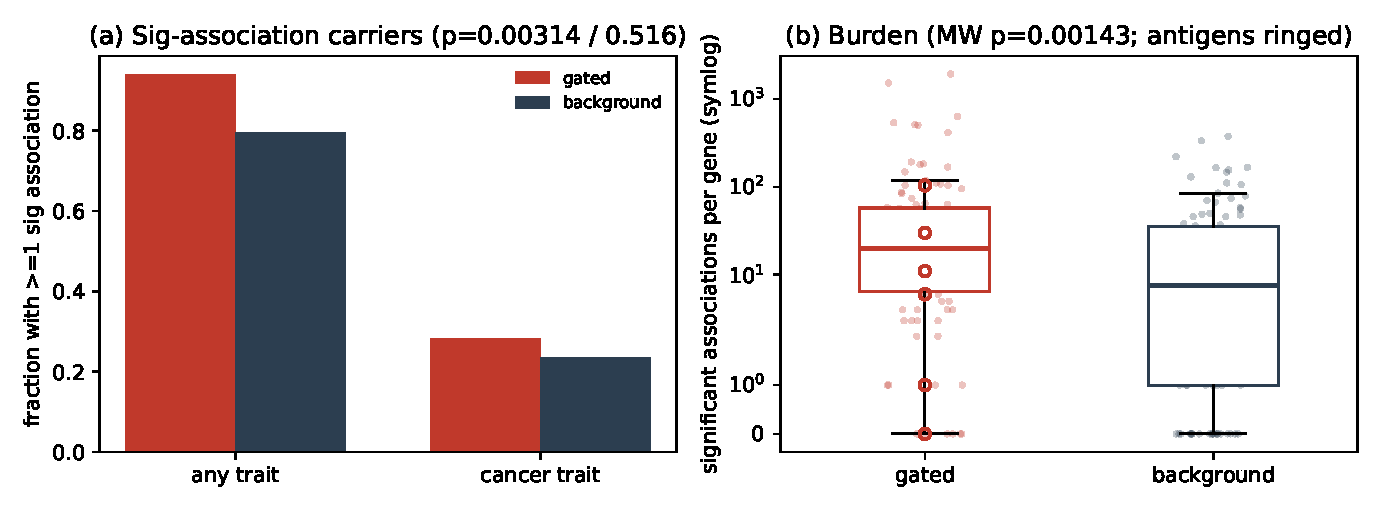
\includegraphics[width=\linewidth]{gwas_fig.pdf}
\caption{GWAS Catalog germline audit. (a) Fraction of genes carrying at
least one genome-wide-significant association, any trait versus cancer
trait. (b) Significant-association burden per gene (symlog axis), with the
seven AND-gate antigens ringed.}
\label{fig:gwas}
\end{figure}
